% Generated from 06-学习型机器人与训练闭环基础.md; edit the LaTeX source after migration.

\part*{第六部分 学习型机器人与训练闭环基础}
\addcontentsline{toc}{part}{第六部分 学习型机器人与训练闭环基础}
\markboth{第六部分 学习型机器人与训练闭环基础}{第六部分 学习型机器人与训练闭环基础}

如果说第五部分说明了机器人为何始终受制于物理、控制与状态估计，那么本部分要回答的则是另一个同样关键的问题：一旦机器人进入学习路线，系统的主要矛盾会如何变化。传统模块化机器人往往把重点放在显式建模、手工接口和结构化工程流程上；学习型机器人则试图把其中一部分能力交给数据驱动方法学习。但这并不意味着问题被简化，相反，它通常把问题重写为另一组更难的对象：数据从哪里来、训练目标如何定义、离线与在线如何衔接、失败样本如何回流、仿真与现实如何迁移，以及系统如何在闭环中持续修正。

因此，本部分并不把模仿学习、强化学习、表示学习和 sim2real 写成互不相干的算法词条，而是把它们统一放在“训练闭环”这一主线上理解。所谓学习型机器人，真正新增的并不只是某个网络结构，而是系统开始依赖一条持续的数据-训练-部署-反馈回流链路来积累能力。也正因为此，学习型机器人既带来了前所未有的泛化可能，也引入了新的脆弱性：covariate shift、数据分布偏移、探索成本、仿真失真、训练目标错配和部署中长尾失败。

\chapter*{27. 模仿学习}
\addcontentsline{toc}{chapter}{27. 模仿学习}
\markboth{27. 模仿学习}{27. 模仿学习}

\section*{27.1 行为克隆}
\addcontentsline{toc}{section}{27.1 行为克隆}


模仿学习之所以长期是机器人学习最现实的起点，不是因为它最“先进”，而是因为它最符合现实数据获取条件。对许多操作任务、移动任务和服务任务而言，最容易拿到的数据并不是大规模在线试错样本，而是人类示教、遥操作轨迹、脚本演示或专家控制记录。行为克隆的基本思想，就是把这些示教轨迹直接转化为监督学习问题：给定观测 \(o_t\)，学习一个策略 \(\pi_\theta\) 输出动作 \(a_t\)。

最基本的训练目标通常写为：

\begingroup
\footnotesize
\begin{equation*}
\min_{\theta} \sum_{t=1}^{T} \lVert \pi_{\theta}(o_t) - a_t^\ast \rVert^2
\end{equation*}
\endgroup

其中，\(a_t^\ast\) 是专家动作。这种写法的优点在于简单直接：不需要显式奖励函数，不需要昂贵探索，也能快速建立一个“会做基本动作”的初始策略。因此，从早期视觉运动策略到今天的大量机器人示教学习系统，行为克隆一直是最自然的入口，代表性工作可参见 \href{https://arxiv.org/abs/1504.00702}{《End-to-End Training of Deep Visuomotor Policies》}。

但行为克隆最核心的脆弱性也非常清楚：训练时看到的是专家状态分布，部署时却会逐步落入策略自己诱发的状态分布。一旦出现微小误差，系统就可能越来越偏离专家轨迹，并在后续时间步中累积放大。这就是学习型机器人里最基本也最重要的 covariate shift 问题。

更形式化地说，行为克隆真正优化的是专家诱导分布上的监督风险，而部署时关心的却是策略自身诱导分布上的长期性能。若把专家分布写成 \(d^{\pi_E}(o)\)，策略分布写成 \(d^{\pi_\theta}(o)\)，则训练目标更接近：

\begingroup
\scriptsize
\begin{equation*}
\mathcal{L}_{\mathrm{BC}}(\theta)=\mathbb{E}_{(o,a^\ast)\sim d^{\pi_E}}\bigl[-\log \pi_\theta(a^\ast \mid o)\bigr]
\end{equation*}
\endgroup

但部署期真正影响成功率的却是：

\begingroup
\footnotesize
\begin{equation*}
J(\pi_\theta)=\mathbb{E}_{o\sim d^{\pi_\theta}}[\text{task success or return}]
\end{equation*}
\endgroup

这两个分布一旦分离，哪怕单步拟合误差很小，也会在闭环滚动中被反复放大。也正因为如此，后来的 DAgger、在线纠偏与失败回流路线，并不是对行为克隆的“可选增强”，而是在正面修补这一分布错位。

\section*{27.2 逆强化学习与偏好学习}
\addcontentsline{toc}{section}{27.2 逆强化学习与偏好学习}


如果把行为克隆理解为“直接模仿专家做了什么”，那么逆强化学习与偏好学习更接近于“推断专家为什么偏好这样做”。二者都试图把人类标准从动作层抬升到目标层，但处理反馈的形式不同。逆强化学习通常假设存在某个隐含奖励函数 \(r_\phi(s, a)\)，专家轨迹之所以优于其他轨迹，是因为它们在该奖励下取得了更高累计回报；偏好学习则不要求先显式恢复完整奖励，而是允许人类只对两段候选行为表达“哪一段更好”，再从成对比较中学习一个可用于排序或训练的偏好模型。

若以轨迹 \(\tau\) 表示一段状态-动作序列，偏好学习常见的最小形式可以写成：

\begingroup
\footnotesize
\begin{equation*}
P(\tau_i \succ \tau_j) = \sigma(f_\phi(\tau_i) - f_\phi(\tau_j))
\end{equation*}
\endgroup

其中 \(f_\phi(\tau)\) 可被视为轨迹奖励或质量评分器。逆强化学习则更强调从专家数据中恢复解释行为的奖励结构，而偏好学习更强调用低成本人类比较信号去拟合“什么叫更好”。对具身系统而言，这种差别很重要，因为很多高质量标准并不是单步动作正确，而是整段行为更平滑、更安全、更符合人类协作习惯。

从工程工作流看，一条典型链路通常是：策略先生成若干候选行为片段，再由人类、规则系统或高可信脚本对片段进行偏好比较，之后训练奖励/偏好模型，最后把它接到离线 RL、重排序器或在线微调回路里。其最小伪代码可以写成：

\begin{lstlisting}[language=python]
segments = collect_candidate_trajectories(policy, env)
labels = query_human_preferences(segments)
reward_model = fit_preference_model(segments, labels)
policy = optimize_policy_with_reward_model(policy, reward_model)
\end{lstlisting}

从工程角度看，逆强化学习与偏好学习的真正价值，不在于它们能神奇地自动发现完美奖励，而在于它们提供了一种把“难以直接写成公式的人类标准”逐步转译进训练目标的机制。对于服务机器人、协作机器人和家庭场景系统，这一点尤其重要，因为很多高质量行为的评价依赖软约束而不是单一成功标签。与此同时，这条路线也有明显代价：偏好标注往往昂贵、主观且受上下文影响；恢复出来的奖励未必具有强可迁移性；一旦数据分布变化，原先学到的偏好结构可能迅速失效。

当人们发现“直接模仿动作”不足以表达复杂任务目标时，就会自然走向另一条思路：不一定模仿动作本身，而是试图恢复驱动这些动作的偏好、代价或奖励结构。逆强化学习的吸引力在于，它试图回答“专家为什么这么做”，而不仅仅是“专家做了什么”。对于同一个高层目标，可能存在多条行为轨迹；若只模仿表面动作，系统容易过拟合于演示细节，而不能抓住真正应优化的任务结构。

偏好学习则进一步把这一思想推向更灵活的人类反馈接口。人类未必总能给出完整专家轨迹，但可以在候选行为之间表达“哪个更好”“哪个更安全”“哪个更自然”。这类方法在具身系统中尤其有意义，因为很多任务的高质量标准并不完全等于“到达目标状态”，还包括接触稳定性、动作平滑性、人机共处安全性和符合现场习惯的执行风格。

\section*{27.3 DAgger 与闭环纠偏}
\addcontentsline{toc}{section}{27.3 DAgger 与闭环纠偏}


DAgger 之所以在模仿学习脉络中如此关键，是因为它清楚指出：如果只在离线专家分布上训练，那么策略在部署时引发的状态偏移会持续累积，因此必须让训练过程看到策略自己会走到的状态，并由专家对这些状态重新标注动作。 其原始论文可参见 \href{https://proceedings.mlr.press/v15/ross11a.html}{DAgger：数据聚合式模仿学习}。

如果把这个思想写成最朴素的流程，就是：

\begin{enumerate}
\item 用专家数据训练初始策略
\item 让当前策略自己运行
\item 在策略实际访问到的状态上收集专家纠正动作
\item 聚合新旧数据重新训练
\end{enumerate}

这件事的重要性，不在于 DAgger 是某个必须逐字复现的算法，而在于它第一次把模仿学习明确推向了闭环训练思路。也就是说，学习型机器人不能只依赖“第一次录好的示教”，而必须把部署中的偏差重新回收到训练中。

\begin{lstlisting}[language=python]
# 示例：DAgger 风格的数据聚合骨架
dataset = initial_expert_dataset()
policy = train_policy(dataset)

for _ in range(num_rounds):
    states = rollout(policy)
    corrections = [expert_action(s) for s in states]
    dataset.extend(zip(states, corrections))
    policy = train_policy(dataset)
\end{lstlisting}

这个片段当然省略了现实中的很多细节，例如部分人工标注、失败回放筛选和安全接管机制，但它说明了一条关键主线：模仿学习一旦认真做下去，就会自然演化成训练闭环问题，而不是静态监督学习问题。

\section*{27.4 示教数据如何塑造具身能力边界}
\addcontentsline{toc}{section}{27.4 示教数据如何塑造具身能力边界}


示教数据并不只是给模型提供“正确答案”，它还在深层上塑造了系统认为哪些动作是正常的、哪些状态是常见的、哪些恢复路径是被允许的。若示教主要来自熟练操作者、固定场景和成功片段，模型学到的往往是干净、规范但覆盖面有限的行为分布；若示教包含更多失败修正、犹豫过程和边界案例，系统更可能获得现实环境中真正有用的恢复性能力。

也因此，示教数据的价值不应只按数量衡量，更应按覆盖的行为边界衡量。很多具身系统后续泛化上限，早在示教采集阶段就已经被决定了一大半。

模仿学习的真正上限，往往不由网络结构决定，而由示教数据的分布、覆盖和质量决定。系统若只见过桌面抓取，就很难自然具备移动操作能力；若只见过成功轨迹，就往往缺少失败恢复能力；若示教本身高度脚本化，则模型即使泛化也更可能泛化到脚本模式，而不是开放世界任务。因此，示教数据并不是“喂给模型的原料”那么简单，而是在很大程度上定义了系统可学会什么、学不会什么、在哪些边界最容易失败。

**工程案例：从离线示教到真机纠偏的策略闭环。** 设想一个视觉条件的抓取与放置技能：团队先用遥操作收集一批正常完成轨迹，训练行为克隆或动作序列策略；随后把候选策略限制在低风险工作区内进行短时试运行，并把抓空、对象滑动、末端错位、因遮挡而停滞等片段单独记录。这个过程的关键不是“上线后多收一点数据”，而是主动让策略进入它自己会诱发的状态分布。DAgger 的理论动机正来自这一点：在序列决策中，后续观测会受前一步动作影响，纯离线监督学习因此容易在自身造成的偏差状态上失效，参见 \href{https://proceedings.mlr.press/v15/ross11a.html}{Ross、Gordon 与 Bagnell 的 DAgger 论文}。

若第 \texttt{\detokenize{k}} 轮试运行收集到的人工纠偏样本为 \(C_k\)，一个受控的数据更新可以写成：

\begingroup
\scriptsize
\begin{equation*}
\mathcal{D}_{k+1} = \mathcal{D}_k \cup \operatorname{filter}(C_k),
\qquad \pi_{k+1} = \operatorname{train}(\mathcal{D}_{k+1})
\end{equation*}
\endgroup

这里的 \texttt{\detokenize{filter}} 不是简单删除坏数据，而应至少区分可恢复偏差、高风险事件、传感异常和标注错误。以动作扩散路线为例，\href{https://www.roboticsproceedings.org/rss19/p026.pdf}{Diffusion Policy} 将视觉条件、动作序列生成和滚动时域执行结合起来，适合说明策略可以输出一段候选动作而非单步命令；但它并不改变上述工程事实：若回流样本没有时间对齐、失败类别和上线条件，模型只会把现场噪声重新编码进策略。

一个可运行的闭环至少需要四道质量门：第一，离线保留集不仅看平均成功率，还要包含偏差状态与恢复片段；第二，仿真或影子执行检查动作是否越过已知安全边界；第三，真机以受限场景灰度运行，并保留人工接管；第四，版本更新后对旧任务做回归测试，防止局部补丁造成已部署技能退化。这个案例说明的是“训练闭环为何必要”，不能据此推出任何一种策略范式在所有任务、本体或接触条件下都更可靠。

\chapter*{28. 强化学习}
\addcontentsline{toc}{chapter}{28. 强化学习}
\markboth{28. 强化学习}{28. 强化学习}

\section*{28.1 MDP 与策略学习基础}
\addcontentsline{toc}{section}{28.1 MDP 与策略学习基础}


对机器人而言，MDP 的真正作用并不是把现实世界“简化成五元组”，而是强迫研究者明确哪些量被当作状态、哪些量被当作动作、奖励究竟偏向结果还是过程、以及策略更新究竟是在拟合什么行为因果链。很多路线争论表面看发生在算法层，实质上却是 MDP 设定不同：有的系统把恢复动作写进动作空间，有的把失败后重试外包给执行器；有的把安全作为硬约束，有的只把它当作奖励惩罚项。只要这层问题没说清，后续任何“算法更强”的比较都很容易失真。

强化学习之所以吸引机器人领域，是因为它看起来提供了一种比模仿学习更自主的能力形成机制：系统不必只复制专家，而可以通过与环境交互优化长期回报。其最经典的问题设定是马尔可夫决策过程：

\begin{equation*}
\mathcal{M} = (\mathcal{S}, \mathcal{A}, P, r, \gamma)
\end{equation*}

其中，状态 \(s_t\)、动作 \(a_t\)、转移概率 \texttt{\detokenize{P}}、奖励 \texttt{\detokenize{r}} 和折扣因子 \(\gamma\) 定义了一条长期决策问题。策略学习的目标通常写为最大化期望累计回报：

\begingroup
\footnotesize
\begin{equation*}
J(\pi) = \mathbb{E}_{\pi}\left[\sum_{t=0}^{T} \gamma^t r_t \right]
\end{equation*}
\endgroup

这一目标的吸引力在于，它允许系统为了长期任务完成度而不是单步模仿精度去优化行为。对于抓取、步态稳定、动态控制和长时程任务，强化学习因此提供了比行为克隆更自然的闭环优化视角。

\section*{28.2 在线 RL 与离线 RL}
\addcontentsline{toc}{section}{28.2 在线 RL 与离线 RL}


在线 RL 与离线 RL 的区别，不只是“是否接触环境”，而是策略更新是否持续依赖新采样数据。在线 RL 假设策略 \(\pi_\theta\) 在训练过程中不断与环境交互，采样新轨迹、估计价值、再更新策略；离线 RL 则固定在一个已经记录好的数据集 \(\mathcal{D}\) 上学习，训练期间不再假设可以无限制获得新样本。对现实机器人而言，这个区别极其关键，因为真机交互昂贵、缓慢、易损且存在安全边界。

若把两者写成最小流程，在线 RL 更像：

\begin{lstlisting}[language=python]
for step in range(K):
    trajectories = rollout(policy, env)
    critic = update_value_function(critic, trajectories)
    policy = improve_policy(policy, critic, trajectories)
\end{lstlisting}

离线 RL 则更像：

\begin{lstlisting}[language=python]
dataset = load_logged_robot_data()
for step in range(K):
    batch = sample(dataset)
    critic = update_value_function(critic, batch)
    policy = conservative_policy_improvement(policy, critic, batch)
\end{lstlisting}

这两条路线面对的问题完全不同。在线 RL 的主要挑战是探索成本、样本效率与安全约束；离线 RL 的主要挑战是分布外动作带来的价值误估。也正因如此，机器人中的离线 RL 常常不会做“自由策略改进”，而会加入保守约束，要求策略不要偏离数据分布太远。现实系统因此普遍采用“离线预训练 + 有限在线校正”的折中流程。

若把离线 RL 的核心困难进一步形式化，可以理解为：评论器 \(Q(s,a)\) 必须在只见过数据集 \(\mathcal{D}\) 的条件下，为策略可能提出的新动作给出估值。一旦对分布外动作过于乐观，策略优化就会朝着“数据里从未真正支持过”的危险区域漂移。以 Conservative Q-Learning 为代表的一类方法，会在 Bellman 误差之外显式加入“压低分布外动作价值”的保守项，典型目标可写为：

\begingroup
\scriptsize
\begin{equation*}
\min_Q \underbrace{\mathbb{E}_{(s,a,r,s')\sim\mathcal{D}}\left[\left(Q(s,a)-\mathcal{B}^{\pi}Q(s,a)\right)^2\right]}_{\text{Bellman 误差}}
+ \alpha\left(\mathbb{E}_{s\sim\mathcal{D},\,a\sim\mu(\cdot\mid s)}[Q(s,a)]-\mathbb{E}_{(s,a)\sim\mathcal{D}}[Q(s,a)]\right)
\end{equation*}
\endgroup

其中 \(\mu(\cdot\mid s)\) 表示某个更宽的候选动作分布，第二项的作用是主动降低“数据没有支撑的动作”在 \(Q\) 函数中的估值，相关代表性工作可参见 \href{https://arxiv.org/abs/2006.04779}{《Conservative Q-Learning for Offline Reinforcement Learning》}。从机器人角度看，这个保守项的意义不是让算法显得更复杂，而是把“不要在纸面上幻想一个现实里并不可靠的动作”直接写进优化目标。

但强化学习一进入真实机器人，就会立刻遭遇现实约束。在线 RL 的理想图景是系统自己在环境中反复试错，但真实机器人中的试错是昂贵的、慢的，而且可能造成磨损、碰撞或安全风险。因此，机器人领域长期非常依赖仿真环境、历史缓冲区、示教初始化和离线数据集。于是，RL 很快就分化为两条路线：一条强调直接在线交互优化，另一条强调在已有数据上做离线策略学习，再辅以有限在线修正。

这一分化本身就说明，机器人中的 RL 从来不是“让机器人自己学一切”那么简单，而是始终要在探索收益与现实代价之间做工程折中。

\section*{28.3 层级强化学习}
\addcontentsline{toc}{section}{28.3 层级强化学习}


层级强化学习可以被视作“把长时程控制问题拆成多个不同时间尺度上的决策器”。最经典的结构是高层管理器和低层执行器：高层每隔若干步产出一个子目标、技能索引或 option，低层则在更高频率上执行连续控制，努力把系统带到该子目标附近。

若把这一结构写成统一抽象，可以得到：

\begin{equation*}
g_t = \pi_H(s_t), \qquad a_t = \pi_L(s_t, g_t)
\end{equation*}

其中 \(g_t\) 是高层在慢时间尺度上给出的子目标或技能标签，\(\pi_L\) 是条件于子目标的低层策略。它们回答的是同一个问题：如何避免让单层策略同时承担“长时程意图规划”和“短时程稳定控制”两类职责。

一个极简工作流可以写成：

\begin{lstlisting}[language=python]
goal = high_level_policy(state)
for _ in range(skill_horizon):
    action = low_level_policy(state, goal)
    state, reward = env.step(action)
    if reached(goal, state):
        break
\end{lstlisting}

这个结构之所以在具身系统里格外自然，是因为真实机器人本来就具有多层时间尺度。语言指令和任务阶段往往以秒级或十秒级变化，而关节控制、接触稳定和避障修正通常是毫秒级到百毫秒级问题。层级 RL 的意义，就是试图让学习系统也尊重这种物理时间结构，而不是把所有决策都塞进同一个平面里。 层级结构的关键收益，在于它把原本难以直接优化的长时程信用分配问题拆成多个较短决策链路。高层不必在每个控制周期都重新决定末端执行器如何运动，而可以在更慢时间尺度上决定当前应激活哪类技能、追求哪个局部目标。低层则专注于在受限上下文中完成局部控制最优化。对于具身任务，这种分离通常不仅提升样本效率，也更方便插入人类先验、安全约束和程序化结构，因此它在后来的 VLA、行为树、技能图谱和程序化规划中不断以不同形式重现。

随着任务变长、状态空间变大、动作结构变复杂，单层策略很难同时处理高层子目标分解与低层连续控制。因此，层级强化学习自然出现：高层策略选择子目标或技能，低层策略负责具体执行。这条路线对具身智能后续的“技能库”“大小脑分层”“程序化中间表示”极具启发性，因为它说明学习系统也会自然走向分层，而不是无限维持单一平面策略。

\section*{28.4 安全强化学习}
\addcontentsline{toc}{section}{28.4 安全强化学习}


安全强化学习之所以在机器人里必须单列，是因为传统 RL 默认的“多试错、多探索”在真实系统中成本极高。机器人每一次危险动作都可能对应硬件损伤、人身风险、现场停线或数据污染，因此安全不能只作为奖励函数里的一项惩罚项，而往往要进入约束、屏障、动作裁剪和人类接管机制中。

这也意味着，机器人中的安全 RL 更像是“在可接受风险边界内学习”，而不是“先任意学习、后再部署”。很多看似降低探索自由度的安全机制，恰恰是让真实学习能够持续进行的必要前提。 这一点之所以需要单独强调，是因为不少关于 RL 的乐观叙事默认了“只要探索足够多，策略总会变好”。但在真实机器人里，不安全探索不仅意味着训练成本增加，还可能直接损坏设备、破坏环境或伤及人员。因此，安全 RL 在具身场景中更像是一套训练制度，而非单一算法名词。它要求我们同时设计奖励、约束、监控、回退和人工接管机制，并承认某些状态区域根本不允许被自由探索。

机器人中的 RL 还必须面对一个纯软件智能体不那么尖锐的问题：探索本身可能带来真实物理风险。因此，安全强化学习并不是附属分支，而几乎是机器人 RL 的默认前提。很多现实系统不得不通过动作裁剪、约束优化、shielding、风险敏感回报和人类接管来限制探索空间，否则训练过程本身就会不可接受。

若把这一问题写成更标准的受约束优化形式，机器人里的安全 RL 往往更接近 constrained MDP，而不是普通 MDP：

\begingroup
\footnotesize
\begin{equation*}
\max_{\pi} J_r(\pi)
\quad \text{s.t.} \quad
J_c(\pi) \le d
\end{equation*}
\endgroup

其中 \(J_r(\pi)\) 表示任务回报，\(J_c(\pi)\) 表示碰撞、超力矩、越界、温升或人机接近风险之类的成本累计，\(d\) 表示允许上界。其拉格朗日形式可写成：

\begingroup
\footnotesize
\begin{equation*}
\mathcal{L}(\pi,\lambda)=J_r(\pi)-\lambda\bigl(J_c(\pi)-d\bigr), \qquad \lambda \ge 0
\end{equation*}
\endgroup

这类写法的重要性在于，它把“安全不是偏好，而是硬边界”明确进了问题定义。像 \href{https://arxiv.org/abs/1705.10528}{《Constrained Policy Optimization》} 这样的工作之所以长期被反复引用，不只是因为它提供了一个算法名字，而是因为它把“每次更新都不能把系统推到明显更危险的区域”这一工程直觉，转写成了可分析、可实现的策略更新约束。对真实机器人而言，shielding、动作裁剪、工作空间屏蔽和安全接管，很多都可以视为这个 constrained MDP 视角在系统层的工程展开。

\section*{28.5 为什么 RL 在机器人里既重要又常被高估}
\addcontentsline{toc}{section}{28.5 为什么 RL 在机器人里既重要又常被高估}


RL 之所以重要，是因为它为机器人提供了一种超越纯示教模仿的路径，使系统能够通过交互优化长期回报、探索策略改进空间并在某些接触与顺序任务上学到人类示教之外的行为结构。尤其在仿真中，RL 仍是许多控制技能与策略优化工作的核心工具。

但 RL 又常被高估，是因为它在论文与视频里常常代表能力上限，而在真实部署中却很难单独承担整套系统能力。真实世界中的数据效率、探索风险、分布漂移、维护成本和奖励设计难题，都使得 RL 更适合作为系统中的一层能力来源，而不是总被浪漫化为万能学习范式。

强化学习在机器人中的真实价值，主要体现在它能够对闭环行为进行长期优化，尤其适合那些难以手工设计控制器、但又可以通过回报近似描述目标的任务。\href{https://arxiv.org/abs/1806.10293}{QT-Opt} 的意义正在于此：它并不是证明“机器人会自己学一切”，而是说明当真实交互数据规模足够大时，闭环 RL 可以在抓取这类具体任务上显著提高鲁棒性与恢复能力。

但 RL 也经常被高估。原因并不神秘：奖励设计困难、探索代价高、样本效率低、真实世界训练慢、安全风险高。这意味着 RL 在机器人里更常扮演“局部行为优化器”或“特定子系统能力增强器”的角色，而不是一个能天然吞掉全部系统问题的统一方案。

\chapter*{29. 表示学习与多任务学习}
\addcontentsline{toc}{chapter}{29. 表示学习与多任务学习}
\markboth{29. 表示学习与多任务学习}{29. 表示学习与多任务学习}

\section*{29.1 自监督表示学习}
\addcontentsline{toc}{section}{29.1 自监督表示学习}


自监督表示学习之所以在机器人中重要，是因为真实交互数据昂贵、标注稀缺，而系统却需要从海量未标注轨迹中先学到可压缩、可迁移、可预测的结构。相比直接端到端监督训练，自监督方法更像是在为后续控制、规划与跨任务迁移铺设共同底座。

不过，机器人里的自监督并不能简单照搬纯视觉领域经验。对具身系统而言，有用的表示不仅要“对图像变化敏感”，还要对动作后果、接触状态、对象可操作性和时序连续性敏感。否则，表示也许很适合分类或检索，却未必足够适合驱动决策。

一旦机器人不再只做单一任务，问题就不再只是“当前策略会不会做这件事”，而变成“系统能否从观测中学到跨任务可复用的结构”。这正是表示学习进入机器人主线的原因。自监督学习的吸引力在于，它允许系统在不依赖昂贵逐步标注的情况下，从多模态观测、时序结构和环境互动中学到对后续任务有用的内部表征。

从更长的脉络看，后来的多模态基础模型、VLA 和机器人 foundation models，本质上都建立在一个前提上：系统必须先学会形成比单任务监督标签更稳定、更可迁移的内部状态结构。

这也是为什么本章要把表示学习放在基础模型之前讲。它并不是附属预备知识，而是后续一切“统一接口”“多任务共享”“跨平台迁移”叙事能够成立的前置条件。

\section*{29.2 多任务共享表征}
\addcontentsline{toc}{section}{29.2 多任务共享表征}


多任务共享表征的核心问题，不是“把所有任务放在一起训练”，而是“哪些表征应该共享，哪些表征必须保留任务特异性”。一个典型架构是共享编码器加条件化任务头：视觉、触觉或状态输入先经过共享 backbone 提取通用特征，再由任务 ID、语言指令或上下文变量进行条件化，最后输出不同任务所需的动作、价值或中间状态。

其最小架构可以写成：

\begin{equation*}
z = f_\theta(o), \qquad a = \pi_\psi(z, c)
\end{equation*}

其中 \(o\) 是观测，\(f_\theta\) 是跨任务共享的表征网络，\(c\) 是任务条件，\(\pi_\psi\) 则是条件策略头。若进一步拆开，还可以为不同任务保留不同 heads：

\begin{lstlisting}[language=python]
features = encoder(obs)
action = task_head[task_id](features)
\end{lstlisting}

这类设计之所以重要，是因为机器人中大量任务共享底层结构。例如相机视角、几何约束、物体边界、抓取前的接近动作、接触前的减速策略，往往都可被多个任务复用。如果每个任务都从零训练一个独立表示，数据利用率会非常低；但如果一味强行共享，又会出现任务冲突、负迁移和梯度干扰。

如果每个任务都单独训练一个策略，那么机器人就仍然停留在“很多孤立技能拼接”的阶段。多任务学习的重要性，在于它尝试让多个任务共享一部分表示空间、技能结构和条件化接口。这样做的收益是明显的：样本可以跨任务复用，表征可以更稳定，系统也更容易在新任务上做迁移。

但代价同样明显：任务冲突、梯度干扰、表示坍塌和任务不平衡会迅速出现。因此，多任务共享并不是“任务越多越好”，而是要求系统明确哪些层应该共享、哪些层必须保留任务特异性。

\section*{29.3 通用技能库与技能迁移}
\addcontentsline{toc}{section}{29.3 通用技能库与技能迁移}


因此，技能迁移真正困难的并不是把一个名字复用到另一台机器人，而是保持其前置条件、可观测状态和失败恢复逻辑也能迁移。一个“抓取”技能在双指夹爪、五指灵巧手和吸盘末端之间，表面任务相同，内部却可能依赖完全不同的接触判据与恢复动作。这也是为什么后续很多基础模型路线会强调技能标记、动作块、可调用接口或程序式接口：它们试图把技能从纯轨迹片段提升为“带契约的中层能力对象”，从而让迁移问题变成接口重绑定，而不只是参数复制。 技能迁移的难点在于，一个看似相同的技能在不同本体、不同夹爪、不同摩擦条件和不同任务容错要求下，往往并不等价。也就是说，技能库不是静态的“动作函数仓库”，而更像一组带有适用前提、参数接口和失败模式描述的中层能力对象。后续很多基础模型路线之所以强调技能标记、动作块或程序式接口，本质上都是在寻找一种既保留可学习性、又维持技能可迁移性的中间表示。

当多任务学习进一步发展，就会自然引出“技能库”思想：与其让高层每次都直接输出低层控制，不如先学习一组可复用技能，再由高层按任务调用。这个想法对后文理解 VLA、程序化中间表示和大小脑架构都非常关键，因为现代具身系统常常不是端到端地每次都从头生成所有动作，而是试图在更稳定的技能原语之上组织行为。

从系统角度看，技能库真正提供的是一种中层可复用性。它让系统既不必把一切写死成传统程序，也不必让每次执行都从原始动作开始重新生成，因此是很多现实路线在“可学习性”和“可部署性”之间取得平衡的关键中介。

\section*{29.4 表征学习如何成为后续基础模型的前置条件}
\addcontentsline{toc}{section}{29.4 表征学习如何成为后续基础模型的前置条件}


更一般地说，基础模型之所以能够在机器人中成立，一个前提就是系统已经学会把不同任务、模态和时间尺度的信息压进某种共享表征空间。没有这一步，所谓“大模型统一一切”往往只会停留在输入输出层面的拼接，而无法形成真正可复用的内部结构。因此，把表示学习看成后续基础模型的前史，不只是历史梳理，更是在提醒我们：如果表征层设计得不对，后面再大的模型也可能只是把系统问题放大而不是解决。

Decision Transformer 的重要性，并不只在于它把强化学习（RL）重写成序列建模，而在于它表明：一旦系统开始把轨迹、回报、状态和动作放到统一序列接口中，传统策略学习与更一般的表示学习之间的边界会开始模糊，相关论文可参见 \href{https://arxiv.org/abs/2106.01345}{《Decision Transformer》}。这为后来的 VLA、动作 token 化和多模态统一接口提供了认知上的桥梁。换言之，机器人基础模型并不是凭空出现的，它们依赖的正是此前这些跨任务表示与统一接口思路的持续积累。

\chapter*{30. sim2real 与域适应}
\addcontentsline{toc}{chapter}{30. sim2real 与域适应}
\markboth{30. sim2real 与域适应}{30. sim2real 与域适应}

\section*{30.1 仿真训练的价值}
\addcontentsline{toc}{section}{30.1 仿真训练的价值}


仿真训练的真正价值，并不只是“便宜地多跑实验”，而是在真实硬件成本过高、危险动作不可直接尝试、长尾扰动难以系统组织时，提供一个可控、可重复、可批量扩展的策略形成环境。它让很多本来在真机上难以系统比较的方案，能够先在统一条件下做初筛和快速迭代。

但仿真最有价值的地方，也恰恰要求研究者对其边界保持清醒。仿真不是现实替身，而更像现实前的训练场和过滤器。若把它当作直接等价的能力证明，就会高估策略的真实部署成熟度；若把它当作结构化筛选工具，其价值则非常高。 从研究方法论上看，仿真还承担着“解耦问题”的作用。真实系统中的失败常常由多种因素叠加导致，而在仿真环境中，研究者可以更系统地单独操纵视觉纹理、动力学参数、接触模型、控制延迟和任务扰动，从而辨识究竟是哪一层假设在失效。也正因如此，仿真不是廉价替代品，而是一种结构化实验平台。后续像 NVIDIA Isaac、MuJoCo、Omniverse、Habitat 这类基础设施的重要性，不仅在于“能跑更多实验”，更在于它们塑造了问题被提出和被验证的方式。

只要真实机器人训练成本高、速度慢、风险大，仿真就几乎不可避免。仿真最大的价值，并不是“替代现实”，而是提供一种可大规模、可并行、可控制、可重复的试验环境，使系统能够在其中学习基础行为、验证训练目标和提前暴露明显失效模式。

对这份报告来说，仿真章节的重要作用还在于建立一个判断习惯：凡是仿真结果，都应继续追问它究竟证明了“结构有效”还是“部署可行”。把这两者分开，后续解读很多论文时会稳得多。

\section*{30.2 域随机化与域自适应}
\addcontentsline{toc}{section}{30.2 域随机化与域自适应}


更稳妥的理解方式是把二者看成两种互补策略。域随机化是在训练期主动扩大输入和动力学分布，让策略学会对变化不敏感；域自适应则是在部署前或部署中显式估计“我现在身处哪个域”，并对表征或参数做针对性修正。前者偏向保守覆盖，后者偏向定向补偿。对具身系统而言，很多成功方案并不是二选一，而是先用域随机化获得基础鲁棒性，再用少量真机数据或在线校准做末端收敛，这比单独押注某一条路线更符合现实工程。 域随机化的思想，是主动让训练分布比目标部署分布更“宽”，以换取策略对未见扰动的容忍度；域自适应则更强调学习如何桥接仿真与真实观测之间的表征差异。两者都不是银弹。随机化过弱，泛化无效；随机化过强，策略可能学不到任何稳定结构。自适应若只对视觉层有效，而真实失配主要来自接触动力学和控制延迟，也难以真正解决问题。因此，sim2real 的关键不是套用某个名词，而是识别系统究竟在哪一层发生了跨域断裂。

但仿真与现实之间从来不存在天然无缝映射。视觉纹理、光照、接触摩擦、执行器延迟、传感器噪声、对象分布和环境扰动都可能发生偏移。因此，sim2real 路线通常需要通过域随机化、域自适应、系统辨识和现实微调来缩小差距。

这里最重要的理解是：sim2real 并不是部署前最后做的一步“小修补”，而是一条贯穿训练早期设计的结构性问题。你在仿真中如何定义任务、如何选状态、如何建奖励、如何建动力学，都会直接影响后续现实部署是否还能成立。

也就是说，sim2real 成败往往早在“问题怎么被表述”这一层就埋下了种子，而不是只在最后迁移那一刻才出现。后文再谈世界模型、基础模型和部署时，都应保留这一视角。

\section*{30.3 现实部署中的失效模式}
\addcontentsline{toc}{section}{30.3 现实部署中的失效模式}


现实部署中的失效模式，往往并不是模型“完全不会做任务”，而是系统在长时程、弱扰动累积和异常边界条件下逐渐暴露脆弱性。例如感知偏移导致抓取点慢慢漂移、策略对某类照明特别敏感、恢复动作在少数边角状态下不可用、或上层计划在连续小误差后失去一致性。

这些失效模式之所以重要，是因为它们更接近真正的运维成本来源。很多系统不是败在第一次任务，而是败在第十次、第一百次和跨场景重复后。理解失效模式，比只关注平均成功率更接近真实部署质量。 从部署复盘角度看，失败模式分析应尽量落到可归责的系统层级。例如，抓取失败究竟是检测框飘移、深度估计偏差、抓取位姿候选错误、接触模型不准，还是末端执行器闭合延迟过大？如果没有这种分层归因，团队就容易把所有失败都模糊归结为“模型泛化不够”，从而错过真正的系统瓶颈。后续报告在评价企业 demo 或学术结果时，也应尽量用这种失效模式框架来判断其工程含金量。

现实中的失效往往不是单点误差，而是多种偏移叠加：视觉模型在新光照下变差，接触模型与真实摩擦失配，控制时延导致原本稳定的轨迹开始振荡，状态估计漂移让策略输入逐步失真。也正因为此，“仿真里会做”从来不能自动推出“现实里能稳定做”。

这类失效模式也说明，部署分析必须尽量落到分层归因，而不是笼统归因为“模型不够泛化”。只有这样，团队才可能知道应该补数据、换接口、加回退，还是重做本体与控制链路。

\section*{30.4 为什么“学得好”不等于“落得下去”}
\addcontentsline{toc}{section}{30.4 为什么“学得好”不等于“落得下去”}


“学得好”与“落得下去”之间的差距，通常不在离线指标本身，而在系统是否能承受真实部署中的分布漂移、执行误差、延迟、异常恢复和维护负担。一个策略在干净数据集、固定起始条件和可控环境中取得高成功率，并不意味着它在连续值班、复杂照明、器件老化或混杂人机协作条件下还能保持稳定表现。

从工程角度看，能否落地更像是在问：模型是否具备足够的恢复能力、是否允许人类低成本接管、是否能通过日志回流形成再训练闭环、以及其错误是否以可管理方式暴露。也正因此，学习系统的真正成熟，往往不是体现在最优片段更惊艳，而是体现在平均运行更稳、失败模式更清晰、维护流程更可复制。

这一定义会贯穿后文对企业和商业化的判断。很多路线不是“不会做”，而是“做了但还不值得交付”；两者差别不在 demo，而在恢复、维护、接管和回流是否成体系。

这一节对全书最重要的意义，在于它提前建立一个判断纪律：学习指标的提升、仿真成绩的提升、离线验证的提升，都不自动等于真实部署能力的提升。后文无论写 VLA、世界模型还是企业 demo，都必须不断回到这一点上检验。

\chapter*{31. 世界模型思想的早期来源}
\addcontentsline{toc}{chapter}{31. 世界模型思想的早期来源}
\markboth{31. 世界模型思想的早期来源}{31. 世界模型思想的早期来源}

\section*{31.1 model-based RL}
\addcontentsline{toc}{section}{31.1 model-based RL}


从算法结构上看，model-based RL 至少包含三个部件：环境模型、规划或想象模块，以及策略/价值更新模块。环境模型试图学习从当前状态和动作到下一状态及奖励的转移关系；规划模块利用该模型在内部试探多个动作后果；策略模块再根据这些“想象经验”或规划结果更新行为。

若以学习得到的动力学模型 \( \hat{P}_\phi(s_{t+1}\mid s_t,a_t) \) 和学习得到的奖励模型 \( \hat{r}_\phi(s_t,a_t) \) 表示环境模型，则最小流程可以写成：

\begin{lstlisting}[language=python]
model = fit_dynamics(real_transitions)
for state in sampled_states:
    imagined_rollouts = rollout_in_model(model, state, candidate_actions)
    score = evaluate(imagined_rollouts)
policy = improve_policy(policy, score)
\end{lstlisting}

这里真正的分水岭，不是“有没有模型”，而是模型在控制链中承担什么角色。有些系统只把模型用于生成辅助训练数据；有些把它用于候选动作排序；有些则把它直接嵌入 MPC 式在线规划。角色不同，对模型精度、稳定性和时延的要求也完全不同。 这一传统的重要性在于，它重新把“预测环境会怎样变化”放回了决策核心。与纯 model-free 路线相比，model-based RL 试图让系统通过内部推演减少真实试错需求，并在规划时显式利用未来状态结构。对于机器人而言，这一点尤其诱人，因为真实交互昂贵而危险；但也正因为如此，任何动力学建模误差都可能被规划过程放大，导致系统在内部想象中看似合理、在现实中却迅速偏离。

从控制视角看，model-based RL 的最大诱惑与最大风险恰好是同一件事：它允许系统把“少量真实样本”扩展成“大量内部推演样本”。如果把模型下的预测回报记为 \(\hat{J}(\pi)\)，真实环境回报记为 \(J(\pi)\)，那么问题的关键不只是让 \(\hat{J}\) 尽量大，而是让 \(|\hat{J}(\pi)-J(\pi)|\) 在候选动作之间保持可控。换句话说，机器人真正需要的不是一套会做漂亮想象的模型，而是一套在比较两个动作序列时，其误差不会把排序彻底颠倒的模型。

世界模型路线之所以值得单独讨论，不是因为它是近两年的新潮名词，而是因为它延续的是更早的 model-based RL 思想：系统不仅学策略，还学习环境动力学或潜在状态演化，再利用这些内部模型进行规划、想象 rollout 或策略优化。

\section*{31.2 潜空间动力学模型}
\addcontentsline{toc}{section}{31.2 潜空间动力学模型}


潜空间动力学模型的标准工作流，通常分为“编码”“潜空间转移”“解码或读出”三步。系统先用编码器把高维观测 \(o_t\) 压缩为潜变量 \(z_t\)，再在潜空间学习转移关系 \(z_{t+1}=f(z_t,a_t)\)，最后按需要解码回观测、奖励、接触属性或价值信号。它与直接像素预测的根本区别在于：模型不再试图重建全部视觉细节，而是希望保留与控制相关的最小充分结构。

一个极简架构可以写成：

\begingroup
\scriptsize
\begin{equation*}
z_t = e_\theta(o_t), \qquad \hat{z}_{t+1} = f_\phi(z_t, a_t), \qquad \hat{o}_{t+1} = d_\psi(\hat{z}_{t+1})
\end{equation*}
\endgroup

如果只关心控制而非重建，最后一步甚至不必显式解码成像素，而可以直接预测奖励、终止标志、接触模式或可供性。也正因为如此，潜空间模型常被进一步区分为“重建导向”和“控制导向”两类：前者更在意观测保真，后者更在意潜变量是否可用于规划、值函数估计和技能切换。 潜空间动力学模型的真正挑战，不只是压缩得足够小，而是要保留对决策真正重要的可控结构。若潜变量只对重建像素有利、却丢失了接触可行性、可达性或物体交互关系，那么它对机器人规划价值有限。反过来，如果潜空间过于任务特化，又会削弱跨任务复用和长期泛化能力。因此，这一层始终处在“表征压缩”与“控制充分性”之间的张力之中，这也是后续世界模型与具身基础模型路线不断分化的根本原因之一。

更严格地说，潜变量 \(z_t\) 的价值不在于“压得够小”，而在于它是否近似构成后续决策所需的充分统计量。一个更接近系统分析的要求是：

\begingroup
\footnotesize
\begin{equation*}
p(o_{t+1}, r_t, c_t \mid h_t, a_t) \approx p(o_{t+1}, r_t, c_t \mid z_t, a_t)
\end{equation*}
\endgroup

其中 \(h_t\) 表示完整历史，\(c_t\) 可以表示接触、终止或约束事件。若这个近似不成立，说明潜变量虽然便于重建，却不足以支撑控制；反之，若它能在较小维度上保留对奖励、接触和可达性的关键条件信息，它才真正有资格成为后续规划与策略优化的工作空间。

一旦观测空间变得高维，直接在像素或原始传感空间中做预测往往代价太高，于是研究者开始学习潜空间表示，并在潜空间中建模动力学。这一步非常关键，因为它把“世界模型”从简单的环境近似，推进成一种“可预测、可规划、可压缩”的内部状态结构。

\section*{31.3 想象 rollout 与规划接口}
\addcontentsline{toc}{section}{31.3 想象 rollout 与规划接口}


“想象 rollout”并不等于简单生成未来画面，它更像是在内部模型中展开一串假设动作，然后把结果交给某种决策接口消费。这个接口可以是动作重排序器、MPC 规划器、价值评估器，或者仅仅是训练时的辅助数据生成器。理解 rollout 的关键，不在于它能否看起来像未来，而在于它与下游控制器之间如何闭环。

最小的 imagination planning 过程可以写成：

\begin{lstlisting}[language=python]
for action_seq in candidate_action_sequences:
    latent = encode(obs)
    returns = 0
    for action in action_seq:
        latent, reward = model.step(latent, action)
        returns += reward
    score[action_seq] = returns
best = argmax(score)
execute(best[0])
\end{lstlisting}

这里可以看出，rollout 的核心是“候选动作序列在模型内的相对排序”，而不是必须得到完美像素视频。对机器人而言，只要内部推演足够帮助区分“更可能成功”和“更可能碰撞或失稳”的候选行为，它就可能有实际价值。 因此，想象 rollout 真正需要回答的问题，不是“能不能生成未来”，而是“生成出来的未来如何以受控方式进入决策接口”。有的系统把它用于价值评估，有的用于动作筛选，有的用于候选计划排序，还有的仅用于离线表征学习。接口不同，世界模型承担的责任也不同。把这一点说清楚很重要，因为它直接决定了我们后文评价世界模型路线时，是把它看成控制器、规划器、数据生成器，还是训练辅助器。

在真实机器人里，这个“受控方式”往往还必须把模型不确定性一并写进去。一个更贴近工程的候选序列评分常写成风险惩罚形式：

\begingroup
\scriptsize
\begin{equation*}
\mathrm{Score}(a_{t:t+H})=
\sum_{\tau=t}^{t+H}\hat{r}_\tau
-\beta \sum_{\tau=t}^{t+H}\mathrm{Uncertainty}(\hat{z}_{\tau})
\end{equation*}
\endgroup

其中第二项并不是锦上添花，而是在提醒系统：内部想象越往长时程展开，模型偏差越可能把“看起来最优”的序列推向现实中的危险区域。也正因为如此，许多世界模型系统真正可用的部分，不是把 rollout 拉得无限长，而是知道在哪个 horizon 截断、在哪些状态拒绝继续相信模型、以及何时把控制权交还给更保守的局部控制器。

\href{https://arxiv.org/abs/1803.10122}{World Models} 与 \href{https://arxiv.org/abs/1912.01603}{Dreamer} 之类工作的重要性，就在于它们明确展示了系统可以在内部模型中做想象 rollout，再据此学习策略或评估未来。对机器人来说，这一思想特别诱人，因为真实试错昂贵，而内部想象似乎提供了一种更高样本效率的替代路径。

但这里也埋下了后文世界模型章节必须正面处理的问题：生成看起来合理的未来，并不等于预测在物理上真实可执行的未来；内部模型可以帮助训练，却不自动保证部署中的稳定性与安全性。

\section*{31.4 为什么世界模型不是凭空冒出来的新潮名词}
\addcontentsline{toc}{section}{31.4 为什么世界模型不是凭空冒出来的新潮名词}


世界模型之所以看上去像一个近年流行的新词，更多是因为它在大模型与生成模型浪潮中重新获得了关注，而不是因为它在机器人与控制中毫无前史。其核心问题始终都在：系统能否通过内部模型预测环境演化、评估动作后果并在执行前进行某种形式的想象式试错。

从这个意义上说，今天的视频世界模型、潜空间 rollout、抽象预测和旧时代的模型预测控制、状态转移建模并不是彼此割裂的宇宙，而是共享同一问题核的不同技术表达。理解这一连续性，有助于避免把许多老问题仅仅因为名字更新就误判为“全新范式”。

因此，本节最重要的作用，是把世界模型重新接回学习型机器人主线。后文如果直接从生成视频或具身基础模型角度谈世界模型，很容易让它显得像一个突然冒出来的新范式；而放回这里看，它其实是基于模型的强化学习、潜空间动力学和想象式规划的继续发展，只是在模型规模和表示能力上被重新放大了。

把这一连续性看清楚，有助于我们避免被术语更新反复带偏。很多今天看似崭新的路线，真正的新意未必在问题本身，而在表示能力、数据规模和接口组织方式上。

\chapter*{本部分小结}
\addcontentsline{toc}{chapter}{本部分小结}
\markboth{本部分小结}{本部分小结}

学习型机器人真正改变的，并不是“机器人开始用神经网络了”这么简单，而是系统能力开始依赖一条持续的训练闭环：示教、交互、反馈、回流、迁移和再训练共同决定系统上限。模仿学习提供现实起点，强化学习提供闭环优化机制，表示学习提供跨任务结构，sim2real 暴露部署断裂，世界模型则尝试把环境动力学重新引入学习链路。

也正因此，本部分与后文的接口非常明确：

\begin{enumerate}
\item 与第 07 部分的接口：表示学习、序列建模和统一接口为大模型进入机器人打基础
\item 与第 10 部分的接口：世界模型并非新概念，而是这里的继续展开
\item 与第 11、13、14 部分的接口：VLA、数据工程、仿真基础设施都建立在这里的训练闭环视角之上
\item 与第 15、16 部分的接口：学习系统的最终价值仍取决于部署约束与安全条件
\end{enumerate}

\chapter*{图表与代码补充}
\addcontentsline{toc}{chapter}{图表与代码补充}
\markboth{图表与代码补充}{图表与代码补充}

本章真正值得反复回看的，不只是单个算法定义，而是它们在训练闭环中的位置关系。若把行为克隆、偏好学习、在线/离线 RL、sim2real 和世界模型放进同一张图里，会更容易看出它们并不是彼此替代的平行名词，而是在回答“数据从哪里来、目标如何定义、策略如何更新、部署偏差如何回流”这几类不同问题。

因此，后续版本中本章的图表应服务于两个稳定目标：第一，把“模仿学习 - RL - 表征学习 - 世界模型”的历史关系画清楚；第二，把“采集 - 训练 - 部署 - 失败回流”的工程闭环画清楚。与其把这些图当作装饰，不如把它们看成本章的结构索引，因为训练型机器人真正新增的就是这条长期数据与能力共演化链路。

代码层面，本章最值得保留的不是大段实现细节，而是几类最小骨架：行为克隆训练循环、离线 RL 的保守更新结构、以及 model rollout 的内部评估回路。它们能帮助读者把抽象术语重新压回到“数据如何进入优化器、优化器如何影响策略、策略又如何回到部署现场”这一条可执行链路上。

\chapter*{图 6-1 学习路线与训练闭环演化图}
\addcontentsline{toc}{chapter}{图 6-1 学习路线与训练闭环演化图}
\markboth{图 6-1 学习路线与训练闭环演化图}{图 6-1 学习路线与训练闭环演化图}

\noindent\textit{源文件：\texttt{\detokenize{assets/diagrams/06-训练闭环演化图.mmd}}}

\begin{figure}[htbp]
\centering
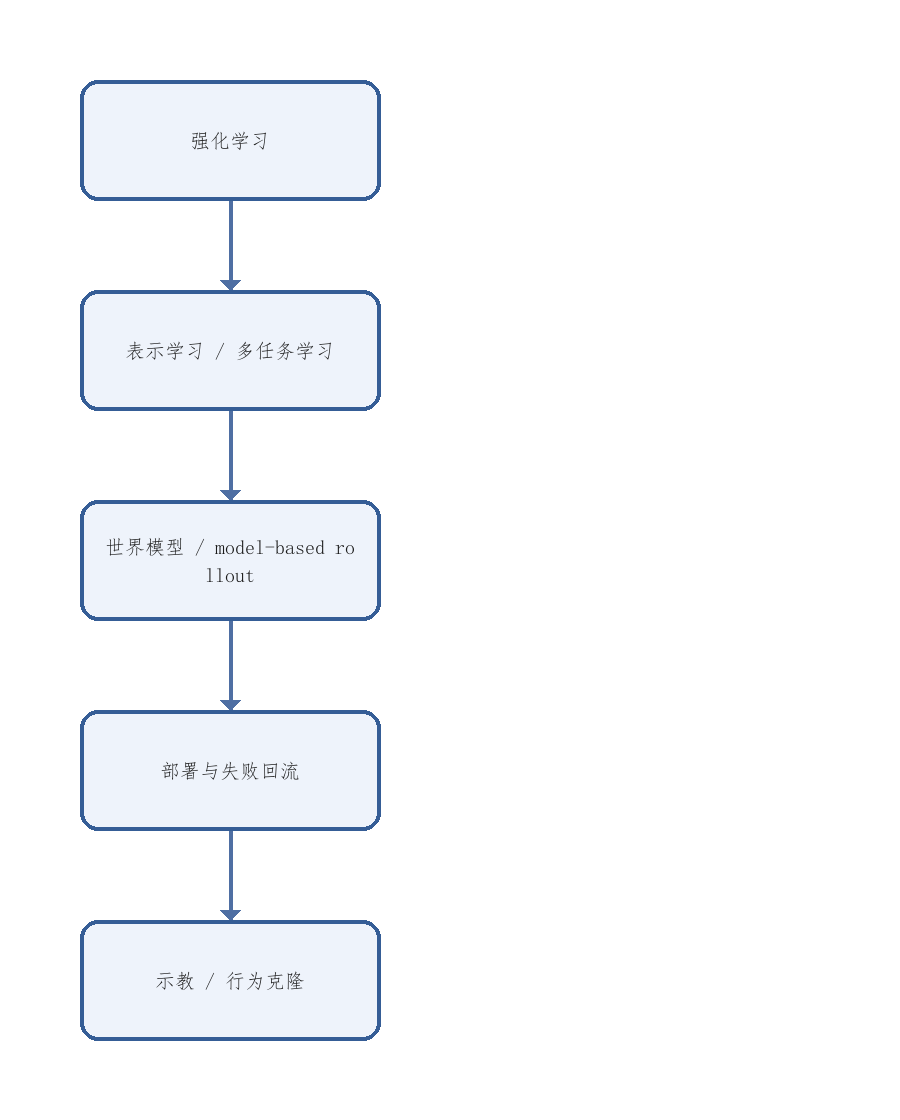
\includegraphics[width=0.9\textwidth,height=0.72\textheight,keepaspectratio]{figures/06-训练闭环演化图.png}
\caption{06-训练闭环演化图}
\label{fig:06-训练闭环演化图}
\end{figure}

\texttt{\detokenize{图 6-1 学习路线与训练闭环演化图}} 的意义，在于把两条经常被分开叙述的主线重新并到一起：一条是“模仿学习 - 强化学习 - 表示学习 - 世界模型”的能力演化主线，另一条是“数据采集 - 训练 - 部署 - 回流”的工程闭环主线。前者解释算法范式如何变化，后者解释这些范式为何会在真实机器人系统中表现出不同的可扩展性；只有把两者放在同一张图里，读者才更容易理解为什么某些训练路线在论文上成立，却在部署上成本极高。

\chapter*{图 6-2 示教策略的闭环纠偏与版本放行}
\addcontentsline{toc}{chapter}{图 6-2 示教策略的闭环纠偏与版本放行}
\markboth{图 6-2 示教策略的闭环纠偏与版本放行}{图 6-2 示教策略的闭环纠偏与版本放行}

\noindent\textit{源文件：\texttt{\detokenize{assets/diagrams/06-闭环纠偏与版本放行图.mmd}}}
\begin{figure}[htbp]
\centering
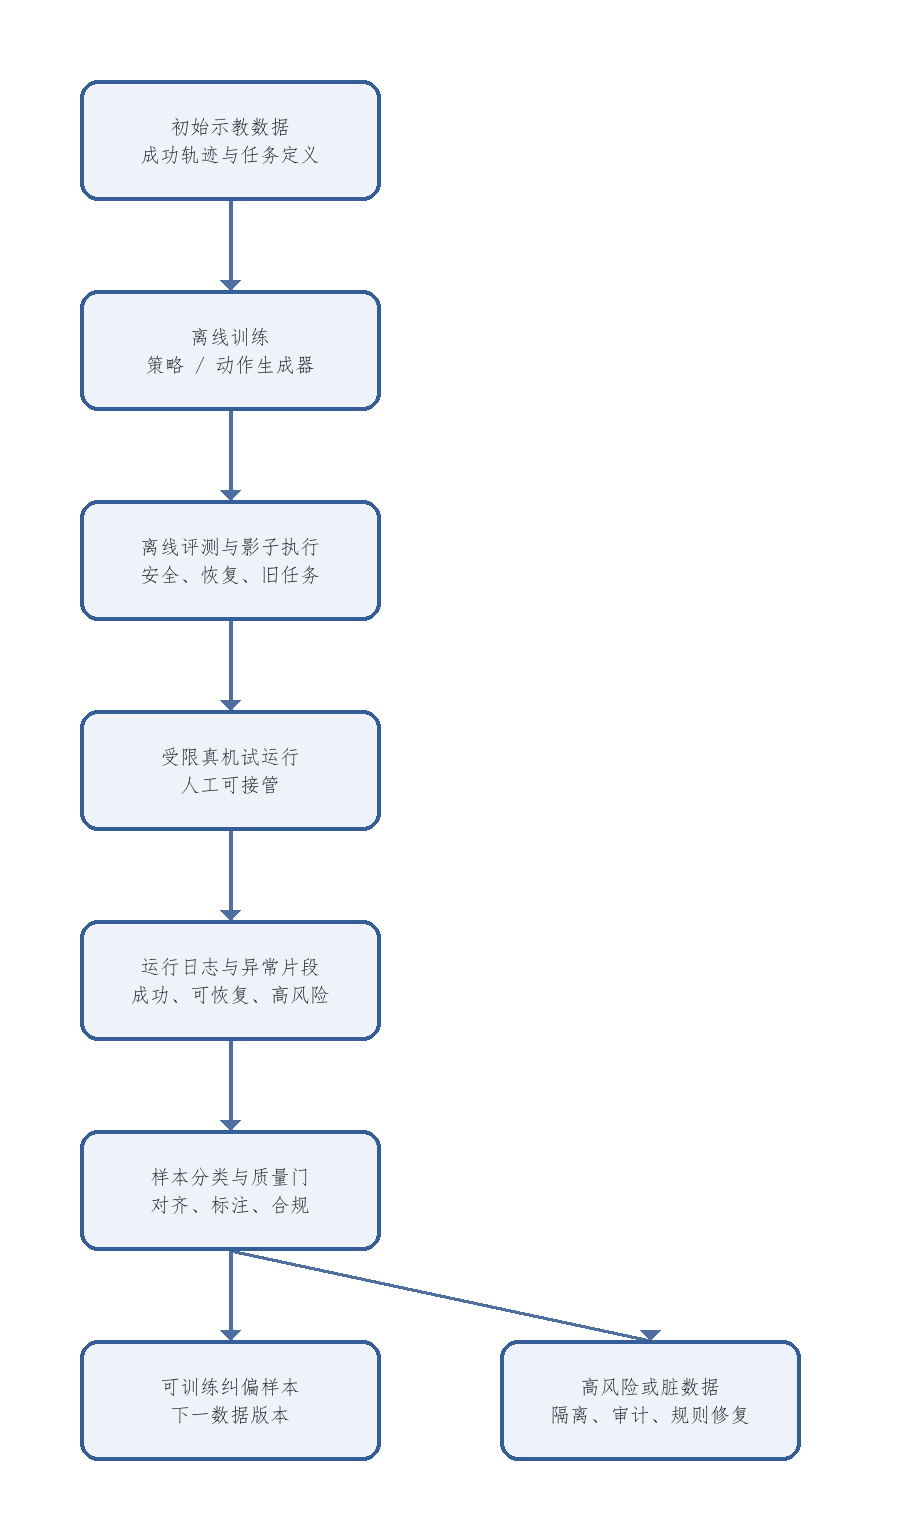
\includegraphics[width=0.9\textwidth,height=0.72\textheight,keepaspectratio]{figures/06-闭环纠偏与版本放行图.png}
\caption{06-闭环纠偏与版本放行图}
\label{fig:06-闭环纠偏与版本放行图}
\end{figure}


\texttt{\detokenize{图 6-2}} 不把“部署回流”画成无条件的自动学习，而是明确插入样本分类、质量门、影子评估和灰度放行。它对应前述案例中的关键判断：失败片段只有在可追溯、可解释且通过安全审查后，才应进入下一轮训练数据。

\chapter*{表 6-1 示教策略闭环纠偏检查表}
\addcontentsline{toc}{chapter}{表 6-1 示教策略闭环纠偏检查表}
\markboth{表 6-1 示教策略闭环纠偏检查表}{表 6-1 示教策略闭环纠偏检查表}

\begingroup
\small
\begin{xltabular}{\textwidth}{YYYYY}
\toprule
阶段 & 最小输入 & 关键检查 & 常见误判 & 进入下一阶段的条件 \\
\midrule
\endfirsthead
\toprule
阶段 & 最小输入 & 关键检查 & 常见误判 & 进入下一阶段的条件 \\
\midrule
\endhead
初始示教 & 任务描述、观察、动作、操作员信息 & 时间同步、任务覆盖、操作质量 & 只保留顺利成功的轨迹 & 能覆盖主路径与常见初始扰动 \\
离线训练 & 固定数据版本与训练配置 & 保留集、动作边界、数据泄漏 & 把训练损失下降当成可部署性 & 通过未见片段与基本安全约束检查 \\
影子评估 & 候选策略与历史日志/仿真 & 偏差状态、恢复动作、旧任务回归 & 只看平均成功率 & 对关键失败模式没有明显回退 \\
真机灰度 & 受限场景、接管接口、运行日志 & 观测时延、接触异常、人工接管次数 & 把一次成功演示视为稳定能力 & 有可追溯的成功、失败与中断记录 \\
回流重训 & 失败分类、纠偏示教、数据版本 & 样本可训练性、风险分层、标注一致性 & 把所有失败同权混入训练集 & 只让通过质量门的样本改变候选策略 \\
\bottomrule
\end{xltabular}
\endgroup

\chapter*{代码 6-1 行为克隆训练骨架}
\addcontentsline{toc}{chapter}{代码 6-1 行为克隆训练骨架}
\markboth{代码 6-1 行为克隆训练骨架}{代码 6-1 行为克隆训练骨架}

\begin{lstlisting}[language=python]
for obs, action_star in dataloader:
    action_pred = policy(obs)
    loss = mse(action_pred, action_star)

    optimizer.zero_grad()
    loss.backward()
    optimizer.step()
\end{lstlisting}

\chapter*{代码 6-2 value update / model rollout 的最小伪代码}
\addcontentsline{toc}{chapter}{代码 6-2 value update / model rollout 的最小伪代码}
\markboth{代码 6-2 value update / model rollout 的最小伪代码}{代码 6-2 value update / model rollout 的最小伪代码}

\begin{lstlisting}[language=python]
latent = encoder(obs)

for step in range(horizon):
    action = actor(latent)
    latent_next, reward = world_model(latent, action)
    target = reward + gamma * value(latent_next)
    value_loss = (value(latent) - target).pow(2).mean()
    latent = latent_next.detach()
\end{lstlisting}

这两段代码分别对应本章最重要的两条学习闭环直觉：一条是“直接模仿已有轨迹”，另一条是“在内部模型里先滚动未来，再反过来更新价值或策略”。
